\begin{tikzpicture}[line cap=round,line join=round]
  \path[use as bounding box] (0,0) rectangle (13.7,10.95);
  \path[pSurface,fill=pBlueWash] (0,5.86) rectangle (6.66,10.82);
  \path[pSurface,fill=pTealWash] (7.04,5.86) rectangle (13.70,10.82);
  \path[pSurface,fill=pGoldWash] (0,.79) rectangle (6.66,5.46);
  \path[pSurface,fill=pResearchWash] (7.04,.79) rectangle (13.70,5.46);
  \pPanel{a}{Structured visual artifacts}{.15}{10.46}
  \pPanel{b}{Images and 3D}{7.19}{10.46}
  \pPanel{c}{Text generation}{.15}{5.10}
  \pPanel{d}{Automated research}{7.19}{5.10}

  % Three representative artifact views per family; all are constructed.
  \node[pTitle,align=center,text width=2.02cm] at (1.11,9.76) {Slides and\\decks};
  \node[pTitle,align=center,text width=2.02cm] at (3.33,9.76) {Webpage\\generation};
  \node[pTitle,align=center,text width=2.02cm] at (5.55,9.76) {Data\\visualizations};
  \path[draw=pBlue!45,fill=pSky!28,rounded corners=2pt]
    (.44,8.26) rectangle (1.90,9.16);
  \path[draw=pBlue!65,fill=white,rounded corners=2pt]
    (.28,8.40) rectangle (1.74,9.30);
  \draw[pBlue,line width=1.5pt] (.42,9.12) -- (1.41,9.12);
  \path[fill=pSky!65,rounded corners=1pt] (.42,8.58) rectangle (.94,8.98);
  \draw[pMuted!55] (1.07,8.93) -- (1.57,8.93)
    (1.07,8.80) -- (1.57,8.80) (1.07,8.67) -- (1.42,8.67);
  \path[draw=pBlue!65,fill=white,rounded corners=3pt]
    (2.47,8.21) rectangle (4.19,9.31);
  \draw[pBlue!40] (2.47,9.10) -- (4.19,9.10);
  \foreach \x in {2.60,2.72,2.84}{\fill[pSky] (\x,9.20) circle (.027);}
  \path[fill=pSky!35,rounded corners=1pt] (2.61,8.35) rectangle (3.13,8.95);
  \draw[pBlue,line width=1.1pt] (3.30,8.89) -- (3.94,8.89);
  \draw[pMuted!55] (3.30,8.72) -- (4.01,8.72) (3.30,8.59) -- (3.87,8.59);
  \path[fill=pSky,rounded corners=1pt] (3.30,8.35) rectangle (3.80,8.46);
  \path[draw=pBlue!40,fill=white,rounded corners=3pt]
    (4.71,8.21) rectangle (6.39,9.31);
  \draw[pMuted!65] (4.92,9.09) -- (4.92,8.39) -- (6.20,8.39);
  \fill[pSky] (5.08,8.39) rectangle (5.30,8.78);
  \fill[pMint] (5.49,8.39) rectangle (5.71,9.05);
  \fill[pPeach] (5.90,8.39) rectangle (6.12,8.88);
  \node[pSmall,align=center] at (1.11,7.72) {Narrative\\and hierarchy};
  \node[pSmall,align=center] at (3.33,7.72) {Fidelity\\and functionality};
  \node[pSmall,align=center] at (5.55,7.72) {Faithful data\\and encodings};
  \draw[pBlue!18] (.22,7.25) -- (6.44,7.25);
  \node[pSmall,text=pInk,anchor=west] at (.24,6.85)
    {Single slides; source- and topic-grounded decks;\\reference- and specification-based web; data-to-chart.};
  \node[pSmall,text=pBlue,anchor=west] at (.24,6.20)
    {Quality depends on both content and its presentation.};

  \node[pTitle,align=center,text width=2.02cm] at (8.15,9.76) {Text-to-image\\generation};
  \node[pTitle,align=center,text width=2.02cm] at (10.37,9.76) {Image\\editing};
  \node[pTitle,align=center,text width=2.02cm] at (12.59,9.76) {Text / image\\to 3D};
  \begin{scope}
    \clip[rounded corners=4pt] (7.31,8.21) rectangle (8.99,9.33);
    \node[inner sep=0pt,anchor=south west] at (7.31,8.21)
      {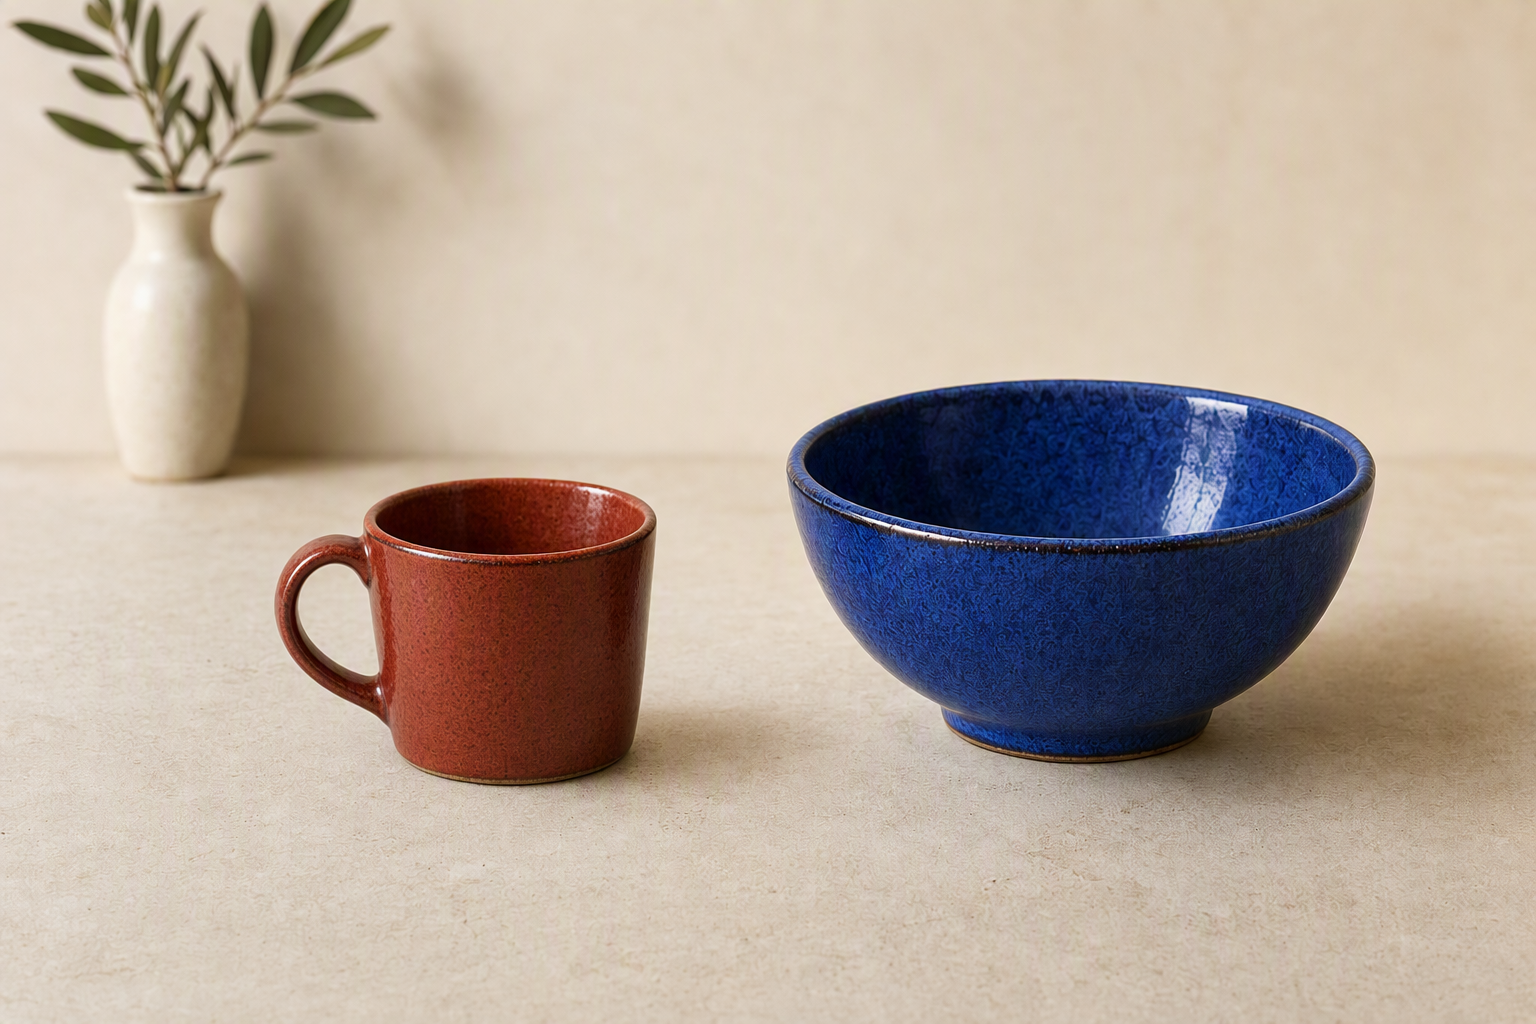
\includegraphics[width=1.68cm]{output/imagegen/edit-preserved.png}};
  \end{scope}
  \path[draw=pTeal!45,fill=white,rounded corners=3pt]
    (9.52,8.21) rectangle (11.22,9.31);
  \path[draw=pBlue,fill=pSky!45] (9.73,8.69) arc[start angle=180,end angle=360,x radius=.24,y radius=.20] -- cycle;
  \draw[pSoftArrow,draw=pTeal] (10.03,8.95) -- (10.50,8.95);
  \path[draw=pBlue,fill=pSky!45] (10.51,8.54) arc[start angle=180,end angle=360,x radius=.22,y radius=.19] -- cycle;
  \path[draw=pResearch,fill=pPeach!75,rounded corners=1pt]
    (10.54,8.75) rectangle (10.86,9.07);
  \draw[pResearch] (10.86,9.00) .. controls (11.05,9.03) and (11.05,8.80) .. (10.86,8.85);
  \pIcon{cube}{pTeal}{12.38}{8.78}{1.22}
  \begin{scope}[shift={(13.03,8.63)},rotate=-13]
    \pIcon{cube}{pTeal}{0}{0}{.69}
  \end{scope}
  \draw[pSoftArrow,draw=pTeal] (12.13,8.17) to[out=-25,in=-155] (13.18,8.15);
  \node[pSmall,align=center] at (8.15,7.72) {Objects\\and relations};
  \node[pSmall,align=center] at (10.37,7.72) {Edit fidelity\\and preservation};
  \node[pSmall,align=center] at (12.59,7.72) {Multi-view\\consistency};
  \draw[pTeal!18] (7.26,7.25) -- (13.48,7.25);
  \node[pSmall,text=pInk,anchor=west] at (7.28,6.85)
    {Also: detailed image captioning and super-resolution.\\Generation and understanding share grounded evidence.};
  \node[pSmall,text=pTeal,anchor=west] at (7.28,6.20)
    {Quality combines grounding with perceptual judgment.};

  \node[pTitle,align=center,text width=2.02cm] at (1.11,4.43) {Document\\summaries};
  \node[pTitle,align=center,text width=2.02cm] at (3.33,4.43) {Grounded\\answers};
  \node[pTitle,align=center,text width=2.02cm] at (5.55,4.43) {Machine\\translation};
  \pIcon{page}{pGold}{.65}{3.45}{1.02}
  \draw[pArrow,draw=pGold] (.98,3.47) -- (1.30,3.47);
  \path[draw=pGold!45,fill=white,rounded corners=3pt]
    (1.37,3.05) rectangle (2.00,3.86);
  \draw[pGold,line width=1.5pt] (1.47,3.67) -- (1.86,3.67);
  \draw[pMuted!50] (1.47,3.48) -- (1.86,3.48) (1.47,3.30) -- (1.79,3.30);
  \pIcon{cards}{pGold}{2.81}{3.46}{.94}
  \draw[pArrow,draw=pGold] (3.23,3.47) -- (3.52,3.47);
  \path[draw=pGold!45,fill=white,rounded corners=3pt]
    (3.60,3.13) rectangle (4.23,3.78);
  \node[pSmall,text=pInk,align=center] at (3.91,3.49) {Text\\{[1]}};
  \path[draw=pGold!45,fill=white,rounded corners=3pt]
    (4.71,3.07) rectangle (5.34,3.90);
  \path[draw=pGold!45,fill=pCream!55,rounded corners=3pt]
    (5.81,3.07) rectangle (6.44,3.90);
  \node[pTitle,text=pGold] at (5.03,3.50) {EN};
  \node[pTitle,text=pGold] at (6.13,3.50) {FR};
  \draw[pArrow,draw=pGold] (5.41,3.49) -- (5.74,3.49);
  \node[pSmall,align=center] at (1.11,2.46) {Faithfulness\\and coverage};
  \node[pSmall,align=center] at (3.33,2.46) {Attribution\\and completeness};
  \node[pSmall,align=center] at (5.55,2.46) {Meaning\\and fluency};
  \draw[pGold!18] (.22,2.01) -- (6.44,2.01);
  \node[pSmall,text=pInk,anchor=west] at (.24,1.59)
    {Also: constraint-following responses and open dialogue.};
  \node[pSmall,text=pGold,anchor=west] at (.24,1.07)
    {Fluent wording can still distort meaning or evidence.};

  \node[pTitle,align=center,text width=2.02cm] at (8.15,4.43) {Research\\ideas};
  \node[pTitle,align=center,text width=2.02cm] at (10.37,4.43) {Ablation\\designs};
  \node[pTitle,align=center,text width=2.02cm] at (12.59,4.43) {Reports\\and reviews};
  \pIcon{flask}{pResearch}{7.86}{3.46}{1.01}
  \path[draw=pResearch!65,fill=pCream!75] (8.56,3.70) circle (.21);
  \draw[pResearch!65] (8.45,3.52) -- (8.45,3.40) -- (8.66,3.40) -- (8.66,3.52);
  \draw[pResearch!55] (8.56,4.01) -- (8.56,4.11)
    (8.84,3.86) -- (8.94,3.92) (8.27,3.86) -- (8.17,3.92);
  \node[pPill,draw=pResearch!45,text=pResearch,minimum width=.83cm] (model)
    at (10.37,3.86) {Model};
  \node[pPill,draw=pResearch!35,text=pResearch,minimum width=.57cm] (on)
    at (9.88,3.09) {on};
  \node[pPill,draw=pResearch!35,text=pResearch,minimum width=.57cm] (off)
    at (10.86,3.09) {off};
  \draw[pArrow,draw=pResearch] (model.south) to[out=-90,in=90] (on.north);
  \draw[pArrow,draw=pResearch] (model.south) to[out=-90,in=90] (off.north);
  \pIcon{page}{pResearch}{12.24}{3.46}{1.13}
  \pIcon{loupe}{pResearch}{12.91}{3.44}{.98}
  \node[pSmall,align=center] at (8.15,2.46) {Novelty\\and testability};
  \node[pSmall,align=center] at (10.37,2.46) {Controlled contrasts\\and confounds};
  \node[pSmall,align=center] at (12.59,2.46) {Inference\\and evidence};
  \draw[pResearch!18] (7.26,2.01) -- (13.48,2.01);
  \node[pSmall,text=pInk,anchor=west] at (7.28,1.59)
    {Also: related-work synthesis and evidence-based critique.};
  \node[pSmall,text=pResearch,anchor=west] at (7.28,1.07)
    {Plausibility alone does not establish a scientific claim.};

  \path[pSurface,fill=pEvoWash] (0,.05) rectangle (13.70,.57);
  \node[pSmall,text=pEvo,align=center] at (6.85,.31)
    {Shared evolution procedure \quad $\vert$ \quad Domain-specific dimensions, priorities, evidence, and human protocols};
\end{tikzpicture}
